\subsection{Aplicación web}

Para el desarrollo de esta  herramienta se ha utilizado \textbf{Java} para el procesamiento de los datos y para diseñar la vista se ha utilizado: \textbf{HTML}, \textbf{CSS} y \textbf{Java server faces}, ademas para conectar el proceso de recolección y clasificación (escritos en \textbf{Python 3}) se hecho uso de \textbf{subprocesos}, los cuales son procesos que corren en segundo plano. En esta sección se explica el proceso de funcionamiento de la aplicación web.\\

La aplicación esta diseñada en 4 módulos ( ver Figura \ref{fig:procesoAppWeb} ): \textbf{Selección} describe las secciones disponibles para obtener noticias; la etapa \textbf{Recolectar} muestra la integración de los \textit{crawlers} en la herramienta; la etapa \textbf{Clasificar} hace uso del modelo clasificador desarrollado en la sección anterior y para concluir, la etapa \textbf{Mostrar resultados} describe la forma en que los datos son presentados al usuario. A continuación se explica a detalla cada una las tareas.


\begin{figure}[h]
	\centering
	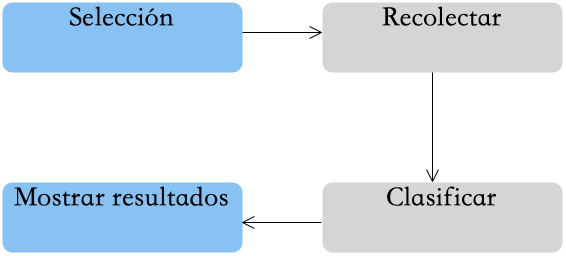
\includegraphics[scale=0.35]{imagenes/Aplicacion/Proceso.png}
	\caption{Etapas de la aplicación web}
	\label{fig:procesoAppWeb}
\end{figure}

\begin{enumerate}
  \item \textbf{Selección de sección}:Esta etapa permite elegir al usuario la sección de noticias a buscar. La aplicación comienza en una pantalla inicial, donde se muestra un menú con las opciones \textbf{Inicio}, \textbf{Cultura}, \textbf{Deportes}, \textbf{Economía}, \textbf{Política}, \textbf{Ciencia y Tecnología}, estas categorías (excluyendo \textbf{Inicio}) son las secciones permitidas para recolectar noticias, como se muestra la el Figura \ref{fig:PantallaInicio}

	\begin{figure}[h]
		\centering
		
\includegraphics[scale=0.18]{imagenes/Aplicacion/pantallaPrincipal.png}
		\caption{Pantalla de Inicio}
		\label{fig:PantallaInicio}
	\end{figure}

 Después de elegir una sección, se muestra el mensaje \textbf{En proceso de recolección y clasificación}, como se visualiza en la Figura \ref{fig:loading}.

	\begin{figure}[h]
	\centering
	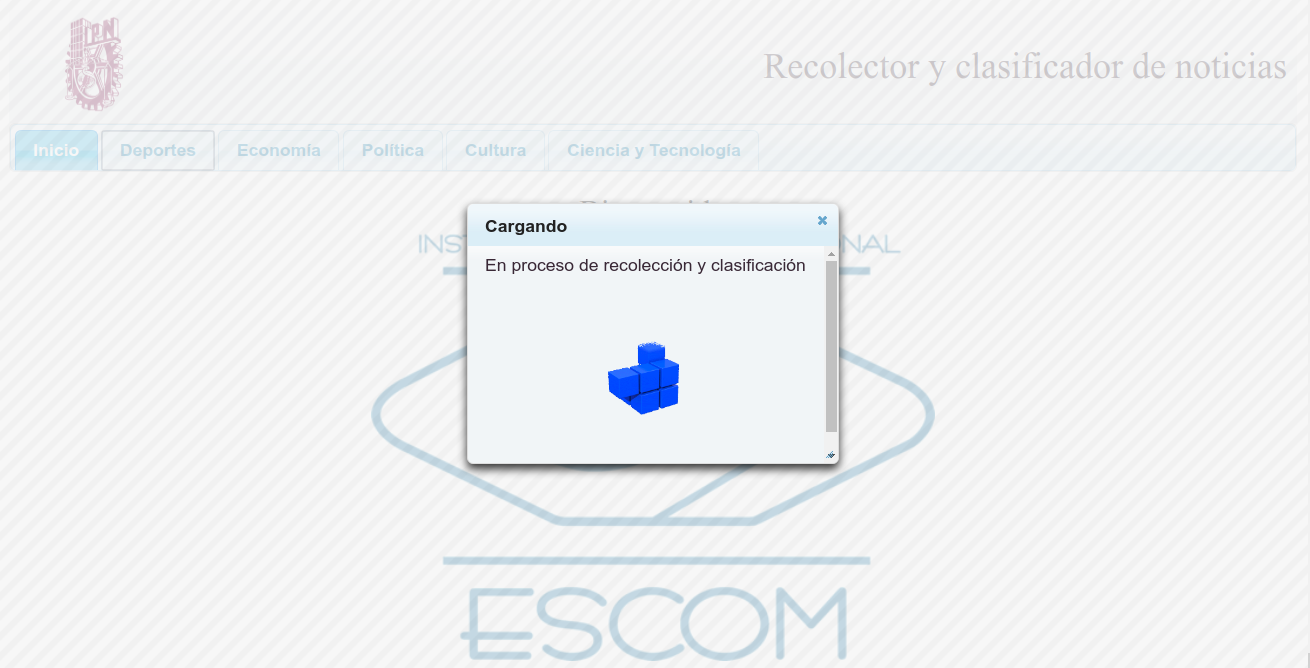
\includegraphics[scale=0.18]{imagenes/Aplicacion/mensajeEspera.png}
	\caption{Mensaje de espera}
	\label{fig:loading}
	\end{figure}


  \item \textbf{Recolección}:Esta etapa genera un subproceso el cual activa un script (desarrollado en \textbf{Python 3}) el cual inicia la recolección de noticias en los sitio web definidos previamente, la información que se obtiene de cada artículo es la siguiente: \textbf{URL de la noticia},\textbf{Título},\textbf{Fecha},\textbf{Autor},\textbf{Descripción} ,\textbf{Noticia}.\\

  La extracción de las noticias se hace en la página principal de los sitios web. Cabe destacar que en el proceso de recolección se valida que las noticias contengan al menos 180 palabras (en la redacción de \textbf{Noticia}), de lo contrario no se extrae. Ademas se ha definido un tiempo máximo de espera en esta etapa, el cual es de 30 segundos, después de concluir el periodo y haber recolectado la información, se procede con la etapa de \textbf{Clasificación}.

  \item \textbf{Clasificación}:Después de recolectar las noticias se inicia la etapa de clasificación, el cual esta conformado por 5 tareas: \textbf{Limpieza}, \textbf{Tokenizar},\textbf{Lematizar}, \textbf{Extracción de características} y \textbf{Clasificar}. Esta etapa genera un subproceso para ejecutar un script desarrollado en \textbf{Python 3}, el cual está encargado de llevar acabo cada tarea de esta sección. Cabe destacar que el proceso de clasificación solo utiliza el contenido de la noticia, los demás datos no son necesarios en esta etapa.

  \item \textbf{Mostrar resultados}:Esta etapa consiste en presentar el resultado del proceso de clasificación en la herramienta. Cuando este proceso ha concluido se muestra el mensaje \textbf{Noticias listas para ser mostradas}, donde el usuario tiene la opción de elegir visualizar las noticias o cancelar el flujo del sistema, como se muestra en la Figura \ref{fig:notClass}. 

	\begin{figure}[h]
		\centering
		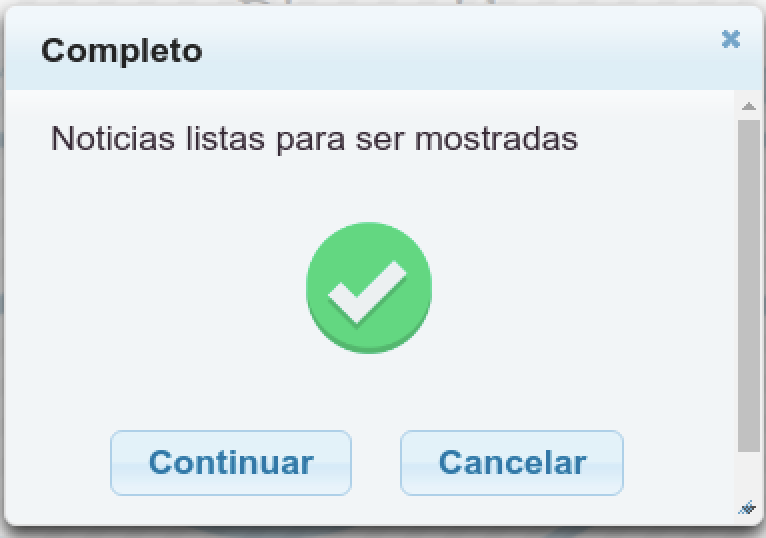
\includegraphics[scale=0.18]{imagenes/Aplicacion/noticiasListasParaSerMostradas.png}
		\caption{Mensaje que se muestra una vez clasificadas las noticias}
		\label{fig:notClass}
	\end{figure}

	Si el usuario ha presionado la opción \textbf{Cancelar}, el proceso concluye y la herramienta muestra la Pantalla de Inicio (ver \ref{fig:PantallaInicio}), de lo contrario si se ha dado clic en \textbf{continuar}, se muestra el resultado de la clasificación, como se muestra en la Figura \ref{fig:vistaNoticias}


	\begin{figure}[h]
	\centering
	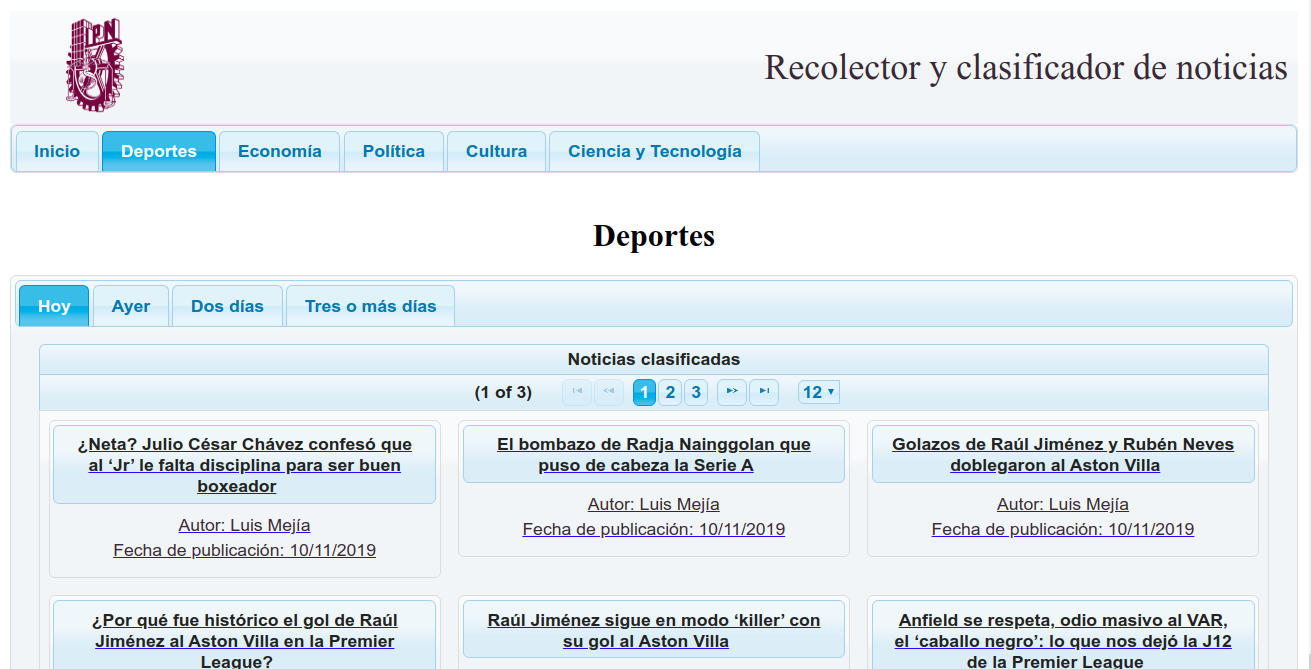
\includegraphics[scale=0.23]{imagenes/Aplicacion/noticiasDeHoy.png}
	\caption{Vista de las noticias recolectadas}
	\label{fig:vistaNoticias}
	\end{figure}
\end{enumerate}
